\documentclass{article}
\usepackage{amsmath, amssymb, tikz}
\usepackage{math}

\title{Introduction to the Theory of Computation \\
    \Large{Chapter 1 Exercises}}
\author{Balachandar Kesavan}
\date{\today}

\begin{document}

\maketitle

\begin{enumerate}
\item
    \begin{enumerate}
    \item
        $q_1$
    \item
        $\set{q_2}$
    \item
        $q_1$
    \item
        $\set{q_1, q_4}$
    \item
        $q_1, q_2, q_3, q_1, q_1$
    \item
        No
    \item
        Yes
    \end{enumerate}
\item
    $ M_1 = (\set{q_1, q_2, q_3}, \set{a, b}, \delta, q_1, \set{q_2}) $ \\
    where $\delta(q_1, a) = q_2, \delta(q_1, b) = q_1, \delta(q_2, \centerdot) = q_3,
    \delta(q_3, a) = q_2, \delta(q_3, b) = q_1$

    $ M_2 = (\set{q_1, q_2, q_3, q_4}, \set{a, b}, \delta, q_1, \set{q_1, q_4}) $ \\
    where $\delta(q_1, a) = q_q, \delta(q_1, b) = q_2, \delta(q_2, a) = q_3,
    \delta(q_2, b) = q_4, \delta(q_3, a) = q_2, \delta(q_3, b) = q_1, \delta(q_4, a)
    = q_3, \delta(q_4, b) = q_4$
\item
    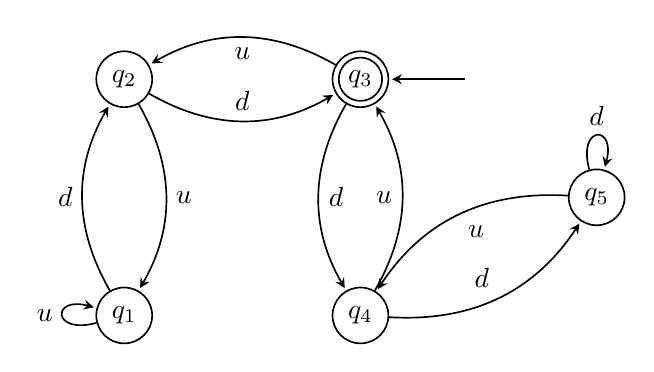
\begin{tikzpicture}
        [->, >=stealth, shorten >=1pt, auto, node distance=2.8cm, semithick]
        \node[shape=circle,draw=black] (q1) at (0, 0) {$q_1$};
        \node[shape=circle,draw=black] (q2) at (0, 3) {$q_2$};
        \node[shape=circle,draw=black] (q3) at (3, 3) {$q_3$};
        \node[shape=circle,draw=black,minimum width=.55cm] (q3accept) at (3, 3) {};
        \node[shape=circle,draw=none] (q3start) at (4.5, 3) {};
        \node[shape=circle,draw=black] (q4) at (3, 0) {$q_4$};
        \node[shape=circle,draw=black] (q5) at (6, 1.5) {$q_5$};

        \path [->] (q3start) edge node {} (q3);

        \path [->] (q1) edge [loop left] node {$u$} (q1);
        \path [->] (q1) edge [bend left] node {$d$} (q2);
        \path [->] (q2) edge [bend left] node {$u$} (q1);
        \path [->] (q2) edge [bend right] node {$d$} (q3);
        \path [->] (q3) edge [bend right] node {$u$} (q2);
        \path [->] (q3) edge [bend right] node {$d$} (q4);
        \path [->] (q4) edge [bend right] node {$u$} (q3);
        \path [->] (q4) edge [bend right] node {$d$} (q5);
        \path [->] (q5) edge [bend right] node {$u$} (q4);
        \path [->] (q5) edge [loop above] node {$d$} (q5);
    \end{tikzpicture}
\item
    \begin{enumerate}
    \item
        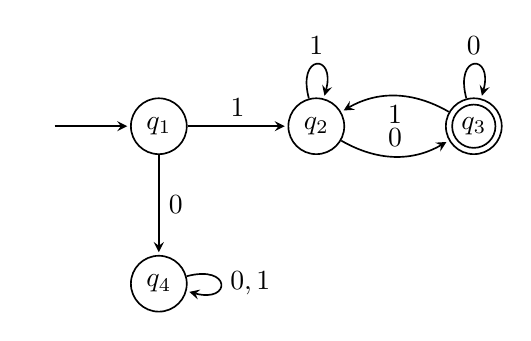
\begin{tikzpicture}
            [->, >=stealth, shorten >=1pt, auto, node distance=2.8cm, semithick]
            \node[shape=circle,draw=black] (q1) at (0, 0) {$q_1$};
            \node[shape=circle,draw=none] (q1start) at (-1.5, 0) {};
            \node[shape=circle,draw=black] (q2) at (2, 0) {$q_2$};
            \node[shape=circle,draw=black] (q3) at (4, 0) {$q_3$};
            \node[shape=circle,draw=black,minimum width=.55cm] (q3accept) at (4, 0) {};
            \node[shape=circle,draw=black] (q4) at (0, -2) {$q_4$};

            \path [->] (q1start) edge node {} (q1);
            \path [->] (q1) edge node {$0$} (q4);
            \path [->] (q1) edge node {$1$} (q2);
            \path [->] (q2) edge [bend right] node {$0$} (q3);
            \path [->] (q2) edge [loop above] node {$1$} (q2);
            \path [->] (q3) edge [loop above] node {$0$} (q3);
            \path [->] (q3) edge [bend right] node {$1$} (q2);
            \path [->] (q4) edge [loop right] node {$0, 1$} (q4);
        \end{tikzpicture}
    \item
        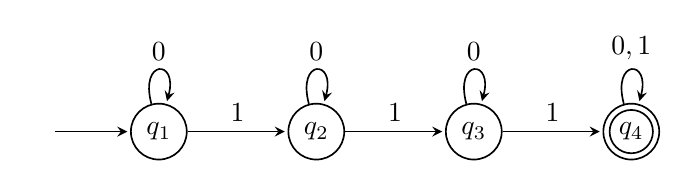
\begin{tikzpicture}
            [->, >=stealth, shorten >=1pt, auto, node distance=2.8cm, semithick]
            \node[shape=circle,draw=black] (q1) at (0, 0) {$q_1$};
            \node[shape=circle,draw=none] (q1start) at (-1.5, 0) {};
            \node[shape=circle,draw=black] (q2) at (2, 0) {$q_2$};
            \node[shape=circle,draw=black] (q3) at (4, 0) {$q_3$};
            \node[shape=circle,draw=black] (q4) at (6, 0) {$q_4$};
            \node[shape=circle,draw=black,minimum width=.55cm] (q4accept) at (6, 0) {};

            \path [->] (q1start) edge node {} (q1);
            \path [->] (q1) edge [loop above] node {$0$} (q1);
            \path [->] (q1) edge node {$1$} (q2);
            \path [->] (q2) edge [loop above] node {$0$} (q2);
            \path [->] (q2) edge node {$1$} (q3);
            \path [->] (q3) edge [loop above] node {$0$} (q3);
            \path [->] (q3) edge node {$1$} (q4);
            \path [->] (q4) edge [loop above] node {$0, 1$} (q4);
        \end{tikzpicture}
    \item
        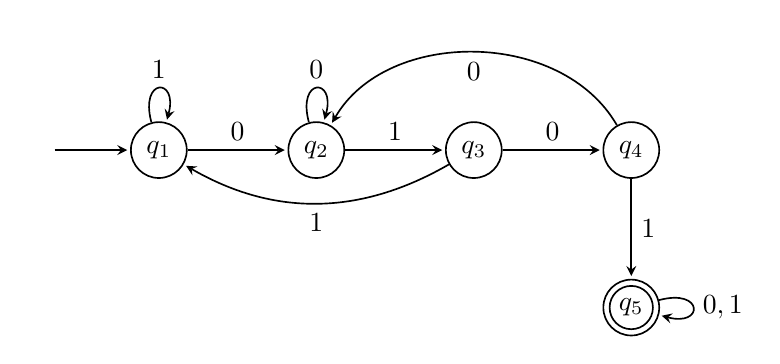
\begin{tikzpicture}
            [->, >=stealth, shorten >=1pt, auto, node distance=2.8cm, semithick]
            \node[shape=circle,draw=black] (q1) at (0, 0) {$q_1$};
            \node[shape=circle,draw=none] (q1start) at (-1.5, 0) {};
            \node[shape=circle,draw=black] (q2) at (2, 0) {$q_2$};
            \node[shape=circle,draw=black] (q3) at (4, 0) {$q_3$};
            \node[shape=circle,draw=black] (q4) at (6, 0) {$q_4$};
            \node[shape=circle,draw=black] (q5) at (6, -2) {$q_5$};
            \node[shape=circle,draw=black,minimum width=.55cm] (q5accept) at (6, -2) {};

            \path [->] (q1start) edge node {} (q1);
            \path [->] (q1) edge [loop above] node {$1$} (q1);
            \path [->] (q1) edge node {$0$} (q2);
            \path [->] (q2) edge [loop above] node {$0$} (q1);
            \path [->] (q2) edge node {$1$} (q3);
            \path [->] (q3) edge [bend left] node {$1$} (q1);
            \path [->] (q3) edge node {$0$} (q4);
            \path [->] (q4) edge [bend right=60] node {$0$} (q2);
            \path [->] (q4) edge node {$1$} (q5);
            \path [->] (q5) edge [loop right] node {$0, 1$} (q5);
        \end{tikzpicture}
    \item
        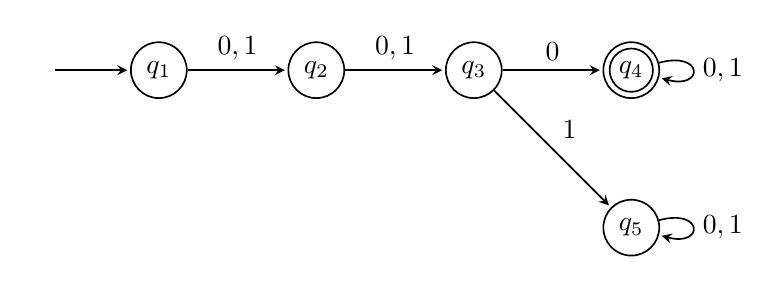
\begin{tikzpicture}
            [->, >=stealth, shorten >=1pt, auto, node distance=2.8cm, semithick]
            \node[shape=circle,draw=black] (q1) at (0, 0) {$q_1$};
            \node[shape=circle,draw=none] (q1start) at (-1.5, 0) {};
            \node[shape=circle,draw=black] (q2) at (2, 0) {$q_2$};
            \node[shape=circle,draw=black] (q3) at (4, 0) {$q_3$};
            \node[shape=circle,draw=black] (q4) at (6, 0) {$q_4$};
            \node[shape=circle,draw=black,minimum width=.55cm] (q4accept) at (6, 0) {};
            \node[shape=circle,draw=black] (q5) at (6, -2) {$q_5$};

            \path [->] (q1start) edge node {} (q1);
            \path [->] (q1) edge node {$0, 1$} (q2);
            \path [->] (q2) edge node {$0, 1$} (q3);
            \path [->] (q3) edge node {$0$} (q4);
            \path [->] (q3) edge node {$1$} (q5);
            \path [->] (q4) edge [loop right] node {$0, 1$} (q4);
            \path [->] (q5) edge [loop right] node {$0, 1$} (q5);
        \end{tikzpicture}
    \item
        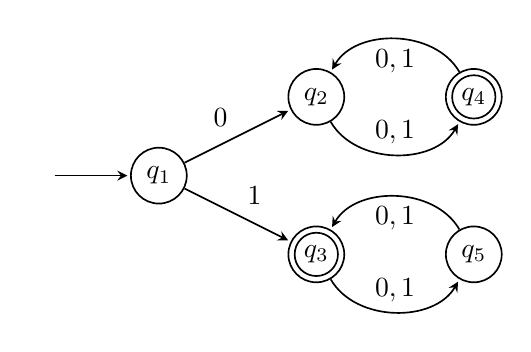
\begin{tikzpicture}
            [->, >=stealth, shorten >=1pt, auto, node distance=2.8cm, semithick]
            \node[shape=circle,draw=black] (q1) at (0, -1) {$q_1$};
            \node[shape=circle,draw=none] (q1start) at (-1.5, -1) {};
            \node[shape=circle,draw=black] (q2) at (2, 0) {$q_2$};
            \node[shape=circle,draw=black] (q3) at (2, -2) {$q_3$};
            \node[shape=circle,draw=black,minimum width=.55cm] (q3accept) at (2, -2) {};
            \node[shape=circle,draw=black] (q4) at (4, 0) {$q_4$};
            \node[shape=circle,draw=black,minimum width=.55cm] (q4accept) at (4, 0) {};
            \node[shape=circle,draw=black] (q5) at (4, -2) {$q_5$};

            \path [->] (q1start) edge node {} (q1);
            \path [->] (q1) edge node {$0$} (q2);
            \path [->] (q1) edge node {$1$} (q3);
            \path [->] (q2) edge [bend right=60] node {$0, 1$} (q4);
            \path [->] (q3) edge [bend right=60] node {$0, 1$} (q5);
            \path [->] (q4) edge [bend right=60] node {$0, 1$} (q2);
            \path [->] (q5) edge [bend right=60] node {$0, 1$} (q3);
        \end{tikzpicture}
    \item
        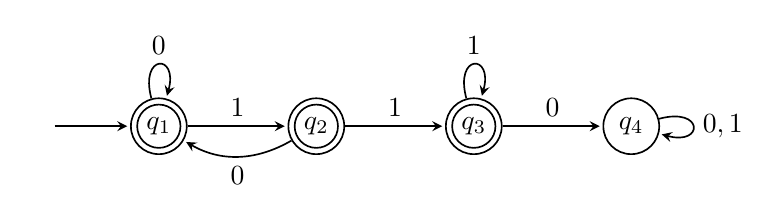
\begin{tikzpicture}
            [->, >=stealth, shorten >=1pt, auto, node distance=2.8cm, semithick]
            \node[shape=circle,draw=black] (q1) at (0, 0) {$q_1$};
            \node[shape=circle,draw=none] (q1start) at (-1.5, 0) {};
            \node[shape=circle,draw=black,minimum width=.55cm] (q1accept) at (0, 0) {};
            \node[shape=circle,draw=black] (q2) at (2, 0) {$q_2$};
            \node[shape=circle,draw=black,minimum width=.55cm] (q2accept) at (2, 0) {};
            \node[shape=circle,draw=black] (q3) at (4, 0) {$q_3$};
            \node[shape=circle,draw=black,minimum width=.55cm] (q3accept) at (4, 0) {};
            \node[shape=circle,draw=black] (q4) at (6, 0) {$q_4$};

            \path [->] (q1start) edge node {} (q1);
            \path [->] (q1) edge [loop above] node {$0$} (q1);
            \path [->] (q1) edge node {$1$} (q2);
            \path [->] (q2) edge [bend left] node {$0$} (q1);
            \path [->] (q2) edge node {$1$} (q3);
            \path [->] (q3) edge [loop above] node {$1$} (q3);
            \path [->] (q3) edge node {$0$} (q4);
            \path [->] (q4) edge [loop right] node {$0, 1$} (q4);
        \end{tikzpicture}
    \item
        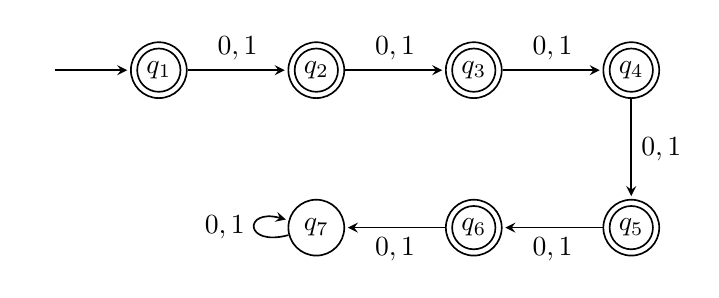
\begin{tikzpicture}
            [->, >=stealth, shorten >=1pt, auto, node distance=2.8cm, semithick]
            \node[shape=circle,draw=black] (q1) at (0, 0) {$q_1$};
            \node[shape=circle,draw=none] (q1start) at (-1.5, 0) {};
            \node[shape=circle,draw=black,minimum width=.55cm] (q1accept) at (0, 0) {};
            \node[shape=circle,draw=black] (q2) at (2, 0) {$q_2$};
            \node[shape=circle,draw=black,minimum width=.55cm] (q2accept) at (2, 0) {};
            \node[shape=circle,draw=black] (q3) at (4, 0) {$q_3$};
            \node[shape=circle,draw=black,minimum width=.55cm] (q3accept) at (4, 0) {};
            \node[shape=circle,draw=black] (q4) at (6, 0) {$q_4$};
            \node[shape=circle,draw=black,minimum width=.55cm] (q4accept) at (6, 0) {};
            \node[shape=circle,draw=black] (q5) at (6, -2) {$q_5$};
            \node[shape=circle,draw=black,minimum width=.55cm] (q5accept) at (6, -2) {};
            \node[shape=circle,draw=black] (q6) at (4, -2) {$q_6$};
            \node[shape=circle,draw=black,minimum width=.55cm] (q6accept) at (4, -2) {};
            \node[shape=circle,draw=black] (q7) at (2, -2) {$q_7$};

            \path [->] (q1start) edge node {} (q1);
            \path [->] (q1) edge node {$0, 1$} (q2);
            \path [->] (q2) edge node {$0, 1$} (q3);
            \path [->] (q3) edge node {$0, 1$} (q4);
            \path [->] (q4) edge node {$0, 1$} (q5);
            \path [->] (q5) edge node {$0, 1$} (q6);
            \path [->] (q6) edge node {$0, 1$} (q7);
            \path [->] (q7) edge [loop left] node {$0, 1$} (q7);
        \end{tikzpicture}
    \item
        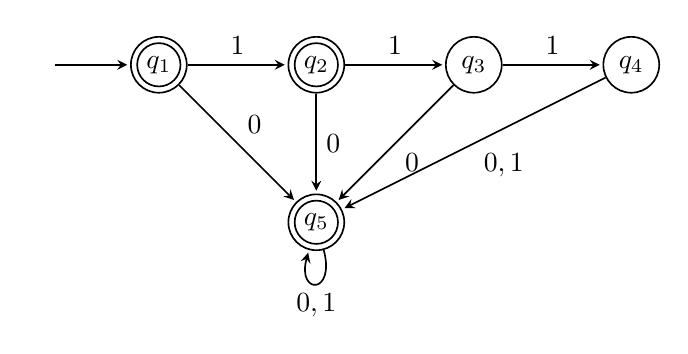
\begin{tikzpicture}
            [->, >=stealth, shorten >=1pt, auto, node distance=2.8cm, semithick]
            \node[shape=circle,draw=black] (q1) at (0, 0) {$q_1$};
            \node[shape=circle,draw=none] (q1start) at (-1.5, 0) {};
            \node[shape=circle,draw=black,minimum width=.55cm] (q1accept) at (0, 0) {};
            \node[shape=circle,draw=black] (q2) at (2, 0) {$q_2$};
            \node[shape=circle,draw=black,minimum width=.55cm] (q2accept) at (2, 0) {};
            \node[shape=circle,draw=black] (q3) at (4, 0) {$q_3$};
            \node[shape=circle,draw=black] (q4) at (6, 0) {$q_4$};
            \node[shape=circle,draw=black] (q5) at (2, -2) {$q_5$};
            \node[shape=circle,draw=black,minimum width=.55cm] (q5accept) at (2, -2) {};

            \path [->] (q1start) edge node {} (q1);
            \path [->] (q1) edge node {$0$} (q5);
            \path [->] (q1) edge node {$1$} (q2);
            \path [->] (q2) edge node {$0$} (q5);
            \path [->] (q2) edge node {$1$} (q3);
            \path [->] (q3) edge node {$0$} (q5);
            \path [->] (q3) edge node {$1$} (q4);
            \path [->] (q4) edge node {$0, 1$} (q5);
            \path [->] (q5) edge [loop below] node {$0, 1$} (q5);
        \end{tikzpicture}
    \item
        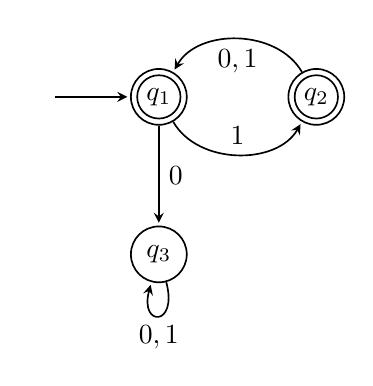
\begin{tikzpicture}
            [->, >=stealth, shorten >=1pt, auto, node distance=2.8cm, semithick]
            \node[shape=circle,draw=black] (q1) at (0, 0) {$q_1$};
            \node[shape=circle,draw=none] (q1start) at (-1.5, 0) {};
            \node[shape=circle,draw=black,minimum width=.55cm] (q1accept) at (0, 0) {};
            \node[shape=circle,draw=black] (q2) at (2, 0) {$q_2$};
            \node[shape=circle,draw=black,minimum width=.55cm] (q2accept) at (2, 0) {};
            \node[shape=circle,draw=black] (q3) at (0, -2) {$q_3$};

            \path [->] (q1start) edge node {} (q1);
            \path [->] (q1) edge node {$0$} (q3);
            \path [->] (q1) edge [bend right=60] node {$1$} (q2);
            \path [->] (q2) edge [bend right=60] node {$0, 1$} (q1);
            \path [->] (q3) edge [loop below] node {$0, 1$} (q3);
        \end{tikzpicture}
    \item
        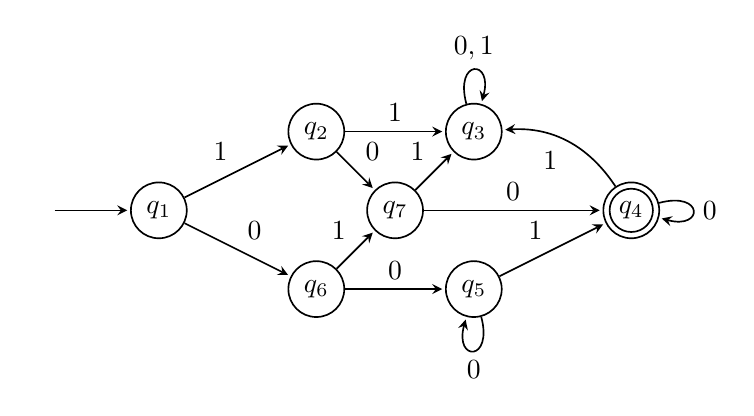
\begin{tikzpicture}
            [->, >=stealth, shorten >=1pt, auto, node distance=2.8cm, semithick]
            \node[shape=circle,draw=black] (q1) at (0, -1) {$q_1$};
            \node[shape=circle,draw=none] (q1start) at (-1.5, -1) {};
            \node[shape=circle,draw=black] (q2) at (2, 0) {$q_2$};
            \node[shape=circle,draw=black] (q3) at (4, 0) {$q_3$};
            \node[shape=circle,draw=black] (q4) at (6, -1) {$q_4$};
            \node[shape=circle,draw=black,minimum width=.55cm] (q4accept) at (6, -1) {};
            \node[shape=circle,draw=black] (q5) at (4, -2) {$q_5$};
            \node[shape=circle,draw=black] (q6) at (2, -2) {$q_6$};
            \node[shape=circle,draw=black] (q7) at (3, -1) {$q_7$};

            \path [->] (q1start) edge node {} (q1);
            \path [->] (q1) edge node {$1$} (q2);
            \path [->] (q2) edge node {$1$} (q3);
            \path [->] (q1) edge node {$0$} (q6);
            \path [->] (q6) edge node {$0$} (q5);
            \path [->] (q2) edge node {$0$} (q7);
            \path [->] (q6) edge node {$1$} (q7);
            \path [->] (q3) edge [loop above] node {$0, 1$} (q3);
            \path [->] (q7) edge node {$1$} (q3);
            \path [->] (q7) edge node {$0$} (q4);
            \path [->] (q5) edge node {$1$} (q4);
            \path [->] (q5) edge [loop below] node {$0$} (q5);
            \path [->] (q4) edge [loop right] node {$0$} (q3);
            \path [->] (q4) edge [bend right] node {$1$} (q3);
        \end{tikzpicture}
    \item
        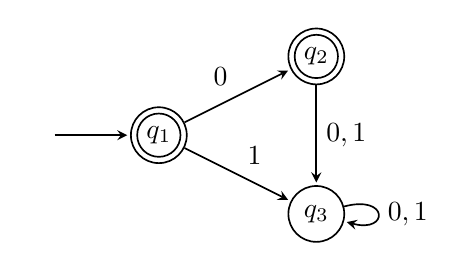
\begin{tikzpicture}
            [->, >=stealth, shorten >=1pt, auto, node distance=2.8cm, semithick]
            \node[shape=circle,draw=black] (q1) at (0, -1) {$q_1$};
            \node[shape=circle,draw=black,minimum width=.55cm] (q1accept) at (0, -1) {};
            \node[shape=circle,draw=none] (q1start) at (-1.5, -1) {};
            \node[shape=circle,draw=black] (q2) at (2, 0) {$q_2$};
            \node[shape=circle,draw=black,minimum width=.55cm] (q2accept) at (2, 0) {};
            \node[shape=circle,draw=black] (q3) at (2, -2) {$q_3$};

            \path [->] (q1start) edge node {} (q1);
            \path [->] (q1) edge node {$0$} (q2);
            \path [->] (q1) edge node {$1$} (q3);
            \path [->] (q2) edge node {$0, 1$} (q3);
            \path [->] (q3) edge [loop right] node {$0, 1$} (q3);
        \end{tikzpicture}
    \item
        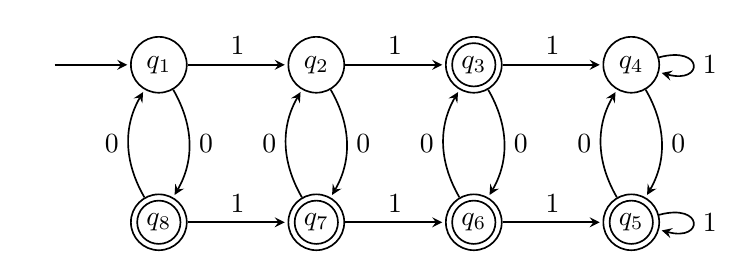
\begin{tikzpicture}
            [->, >=stealth, shorten >=1pt, auto, node distance=2.8cm, semithick]
            \node[shape=circle,draw=black] (q1) at (0, 0) {$q_1$};
            \node[shape=circle,draw=none] (q1start) at (-1.5, 0) {};
            \node[shape=circle,draw=black] (q2) at (2, 0) {$q_2$};
            \node[shape=circle,draw=black] (q3) at (4, 0) {$q_3$};
            \node[shape=circle,draw=black,minimum width=.55cm] (q3accept) at (4, 0) {};
            \node[shape=circle,draw=black] (q4) at (6, 0) {$q_4$};
            \node[shape=circle,draw=black] (q5) at (6, -2) {$q_5$};
            \node[shape=circle,draw=black,minimum width=.55cm] (q5accept) at (6, -2) {};
            \node[shape=circle,draw=black] (q6) at (4, -2) {$q_6$};
            \node[shape=circle,draw=black,minimum width=.55cm] (q6accept) at (4, -2) {};
            \node[shape=circle,draw=black] (q7) at (2, -2) {$q_7$};
            \node[shape=circle,draw=black,minimum width=.55cm] (q7accept) at (2, -2) {};
            \node[shape=circle,draw=black] (q8) at (0, -2) {$q_8$};
            \node[shape=circle,draw=black,minimum width=.55cm] (q8accept) at (0, -2) {};

            \path [->] (q1start) edge node {} (q1);
            \path [->] (q1) edge [bend left] node {$0$} (q8);
            \path [->] (q8) edge [bend left] node {$0$} (q1);
            \path [->] (q2) edge [bend left] node {$0$} (q7);
            \path [->] (q7) edge [bend left] node {$0$} (q2);
            \path [->] (q3) edge [bend left] node {$0$} (q6);
            \path [->] (q6) edge [bend left] node {$0$} (q3);
            \path [->] (q4) edge [bend left] node {$0$} (q5);
            \path [->] (q5) edge [bend left] node {$0$} (q4);
            \path [->] (q1) edge node {$1$} (q2);
            \path [->] (q2) edge node {$1$} (q3);
            \path [->] (q3) edge node {$1$} (q4);
            \path [->] (q4) edge [loop right] node {$1$} (q4);
            \path [->] (q8) edge node {$1$} (q7);
            \path [->] (q7) edge node {$1$} (q6);
            \path [->] (q6) edge node {$1$} (q5);
            \path [->] (q5) edge [loop right] node {$1$} (q5);
        \end{tikzpicture}
    \item
        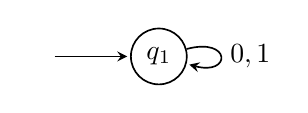
\begin{tikzpicture}
            [->, >=stealth, shorten >=1pt, auto, node distance=2.8cm, semithick]
            \node[shape=circle,draw=black] (q1) at (0, 0) {$q_1$};
            \node[shape=circle,draw=none] (q1start) at (-1.5, 0) {};

            \path [->] (q1start) edge node {} (q1);
            \path [->] (q1) edge [loop right] node {$0, 1$} (q1);
        \end{tikzpicture}
    \item
        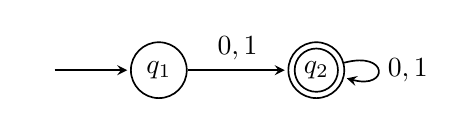
\begin{tikzpicture}
            [->, >=stealth, shorten >=1pt, auto, node distance=2.8cm, semithick]
            \node[shape=circle,draw=black] (q1) at (0, 0) {$q_1$};
            \node[shape=circle,draw=none] (q1start) at (-1.5, 0) {};
            \node[shape=circle,draw=black] (q2) at (2, 0) {$q_2$};
            \node[shape=circle,draw=black,minimum width=.55cm] (q2accept) at (2, 0) {};

            \path [->] (q1start) edge node {} (q1);
            \path [->] (q1) edge node {$0, 1$} (q2);
            \path [->] (q2) edge [loop right] node {$0, 1$} (q2);
        \end{tikzpicture}
    \end{enumerate}
\item
    \begin{enumerate}
    \item
        \todo
    \end{enumerate}
\end{enumerate} 
\end{document}
